\documentclass[hyperref={pdfpagelabels=false}]{beamer}

% A apresentação 'Minicurso de Introdução ao LaTeX' de Wanderson Henrique
% Camargo Rosa foi licenciada com uma Licença Creative Commons - Atribuição -
% Uso Não Comercial - Partilha dos Mesmos Termos 3.0 Não Apropriada

% Pacotes Utilizados -----------------------------------------------------------
\usepackage[utf8]{inputenc}
\usepackage[T1]{fontenc}
\usepackage[brazil]{babel}

% Informações Pessoais ---------------------------------------------------------
\title[\LaTeX{}]{Minicurso de Introdução ao \LaTeX{}}
\author[ROSA]{Wanderson Henrique Camargo Rosa}
\institute[UNISINOS]{Centro de Ciências Exatas e Tecnológicas\\Universidade do
Vale do Rio dos Sinos -- Unisinos}
\date{São Leopoldo, Maio de 2011}
\keywords{uniinfo latex sbc}

% Configurações Gerais ---------------------------------------------------------
\let\Tiny=\tiny
\setbeamertemplate{navigation symbols}{}
\AtBeginSubsection[]
{
\begin{frame}<beamer>
\frametitle{Agenda}
\tableofcontents[currentsection,currentsubsection]
\end{frame}
}

% Documento --------------------------------------------------------------------
\begin{document}

% Título -----------------------------------------------------------------------
\begin{frame}
    \maketitle{}
    \begin{center}
        \includegraphics[scale=0.5]{images/cc}
    \end{center}
\end{frame}

\begin{frame}{Agenda}
    \tableofcontents{}
\end{frame}

% Apresentação -----------------------------------------------------------------
\section{Apresentação}
\label{sec:apresentacao}

\subsection{Sobre o Minicurso}

\begin{frame}{Objetivo}
    Criar um artigo que esteja padronizado conforme as normas da Sociedade
    Brasileira de Computação (SBC), disponibilizadas em pacote específico por
    aquela instituição, utilizando \LaTeXe{} e ferramentas de código aberto.
\end{frame}

\begin{frame}{Aptidões Adquiridas}
    O aluno estará apto a criar um artigo simples segundo normas da SBC
    fornecidas. Também poderá pesquisar conteúdos sobre \LaTeX{} em
    bibliografias exibidas e filtrar informações relevantes durante a busca.
    Capacidade de escrever referências bibliográficas utilizando ferramentas
    auxiliares como o Bib\TeX{}.
\end{frame}

% Introdução -------------------------------------------------------------------
\section{Introdução}
\label{sec:introducao}

\subsection{Histórico}

\begin{frame}{Definição}
    \LaTeX{} é um sistema de composição de textos \cite{oetiker2008}, adequado
    para produção de documentos com alta qualidade tipográfica. É uma versão
    especial do \TeX{} que entende comandos próprios \cite{lamport1994} e
    trabalha buscando dividir as funções de formatação de documentos e a ordem
    lógica do texto.
\end{frame}

\begin{frame}{Donald Knuth e \TeX{}}
    \begin{itemize}
        \item Grande Contribuidor para Computação
        \item Programação Literária
        \item Insatisfeito com Qualidade em Documentos
    \end{itemize}
    \pause{}
    \begin{figure}
        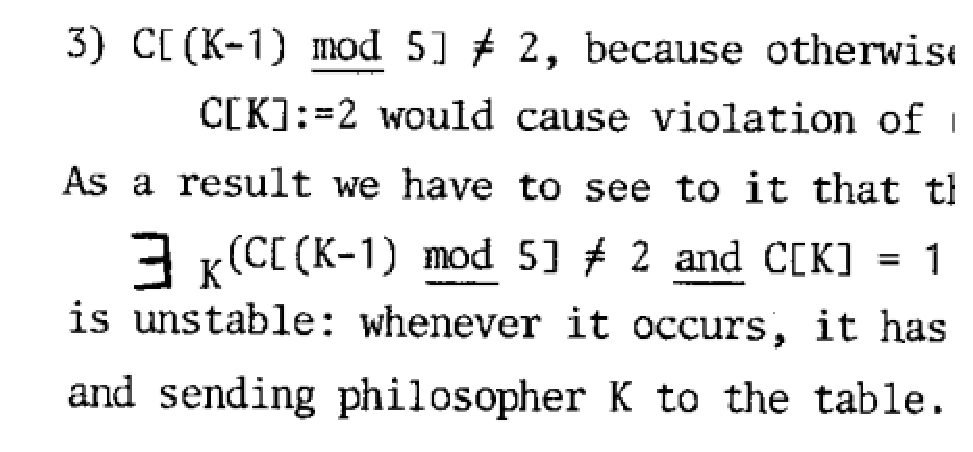
\includegraphics[scale=0.4]{images/dijkstra}
        \caption{Dijkstra e Escalonamento de Processos}
    \end{figure}
\end{frame}

\begin{frame}{Donald Knuth e \TeX{}}
    \begin{columns}[c]
        \begin{column}{0.5\textwidth}
            \begin{figure}
                \centering{}
                \includegraphics[width=\textwidth]{images/knuth}
            \end{figure}
        \end{column}
        \begin{column}{0.5\textwidth}
            \begin{figure}
                \centering{}
                \includegraphics[width=\textwidth]{images/texbook}
            \end{figure}
        \end{column}
    \end{columns}
\end{frame}

\begin{frame}[fragile]{Leslie Lamport e \LaTeX{}}
    \begin{itemize}
        \item Cientista da Computação
        \item Teoria de Sistemas Distribuídos
        \item Dificuldade de Utilização do \TeX{}
    \end{itemize}
    \pause{}
    \begin{block}{Bhaskara}
        \begin{equation*}
            \frac{-b\pm\sqrt{b^2-4ac}}{2a}
        \end{equation*}
        \centering{}
        \verb,\frac{-b\pm\sqrt{b^2-4ac}}{2a},
    \end{block}
\end{frame}

\begin{frame}{Leslie Lamport e \LaTeX{}}
    \begin{columns}[c]
        \begin{column}{0.5\textwidth}
            \begin{figure}
                \centering{}
                \includegraphics[width=\textwidth]{images/lamport}
            \end{figure}
        \end{column}
        \begin{column}{0.5\textwidth}
            \begin{figure}
                \centering{}
                \includegraphics[width=\textwidth]{images/latexbook}
            \end{figure}
        \end{column}
    \end{columns}
\end{frame}

\subsection{Informações}

\begin{frame}{\LaTeX{}}
    \begin{itemize}
        \item Vantagens \cite{oetiker2008}
        \begin{itemize}
            \item Padrões Profissionais;
            \item Suporte Matemático Nativo;
            \item Divisão Lógica do Documento; e
            \item Rodapé, Referências Cruzadas e Índice Automáticos.
        \end{itemize}
        \pause{}
        \item Desvantagens
        \begin{itemize}
            \item Dificuldade para Modificar Formatos;
            \item Escrever Documentos sem Ordem Lógica; e
            \item Aparência Inicial Complicada.
        \end{itemize}
    \end{itemize}
\end{frame}

\begin{frame}{Idéia Principal}
    \LaTeX{} \cite{oetiker2008} habilita o autor do documento a formatar seu
    próprio trabalho com qualidade profissional usando formatos
    \alert{pré-definidos}.
    \pause{}
    \begin{itemize}
        \item Formatos Disponíveis
        \begin{itemize}
            \item Associação Brasileira de Normas Técnicas (ABNT)
            \item Sociedade Brasileira de Computação (SBC)
            \item Muitos Outros!
        \end{itemize}
    \end{itemize}
\end{frame}

\begin{frame}{Ferramentas}{Ambientes de Edição}
    \begin{columns}[t]
        \begin{column}{0.5\textwidth}
            \begin{itemize}
                \item Windows
                \begin{itemize}
                    \item Mik\TeX{}
                    \item \TeX{}nicCenter
                \end{itemize}
            \end{itemize}
            \begin{figure}
                \centering{}
                \includegraphics[scale=0.4]{images/miktex}
            \end{figure}
        \end{column}
        \begin{column}{0.5\textwidth}
            \begin{itemize}
                \item Linux
                \begin{itemize}
                    \item \TeX{}maker
                    \item \TeX{}lipse
                \end{itemize}
            \end{itemize}
            \begin{figure}
                \centering{}
                \includegraphics[scale=0.4]{images/texmaker}
            \end{figure}
        \end{column}
    \end{columns}
\end{frame}

% Documento --------------------------------------------------------------------
\section{Documento}
\label{sec:documento}

\subsection{Texto para Edição}

\begin{frame}[fragile]{Texto para Edição}{Documento Inicial}
    \begin{center}
        \huge{\verb,http://goo.gl/9R5Rm,}
    \end{center}
\end{frame}

\begin{frame}[fragile]{Texto para Edição}{Estrutura de Arquivo}
    \begin{columns}[t]
        \begin{column}{0.5\textwidth}
\begin{verbatim}
\documentclass[opt]{tipo}

% Preâmbulo
% Comentários

\usepackage[opt]{pacote}

\begin{document}

    Texto e Comandos
    \begin{ambiente}
        Texto e Comandos
    \end{ambiente}

\end{document}
\end{verbatim}
        \end{column}
        \begin{column}{0.5\textwidth}
\begin{verbatim}
Classe

Informações do Documento
Comentários com '%'

Carregar Pacote

Início do Documento

Texto
Início de Ambiente
Texto
Fim de Ambiente

Fim do Documento
\end{verbatim}
        \end{column}
    \end{columns}
\end{frame}

\begin{frame}[fragile]{Texto para Edição}{Documento Padrão}
    \begin{columns}[t]
        \begin{column}{0.5\textwidth}
\begin{verbatim}
\documentclass{article}

\usepackage[utf8]{inputenc}
\usepackage[T1]{fontenc}
\usepackage[brazil]{babel}

\begin{document}
    Primeiro Documento!
\end{document}
\end{verbatim}
        \end{column}
        \begin{column}{0.5\textwidth}
\begin{verbatim}
% Tipo do Documento

% [latin1] para Windows
% Codificação de Fontes
% Texto em Português

% Início do Documento

% Fim do Documento
\end{verbatim}
        \end{column}
    \end{columns}
\end{frame}

\subsection{Personalizando}

\begin{frame}[fragile]{Personalizando}{Dados Pessoais}
\begin{verbatim}
\documentclass{article}

\usepackage[utf8]{inputenc}
\usepackage[T1]{fontenc}
\usepackage[brazil]{babel}
\usepackage{sbc-template}

\title{Nome do Artigo}
\author{Nome do Autor}

\begin{document}
    \maketitle{}
    Primeiro Documento!
\end{document}
\end{verbatim}
\end{frame}

\begin{frame}[fragile]{Personalizando}{Resumo}
\begin{verbatim}
\begin{document}

    \maketitle{}

    % Abstract in English
    \begin{abstract}
        Abstract
    \end{abstract}

    % Resumo em Português
    \begin{resumo}
        Resumo
    \end{resumo}

\end{document}

\end{verbatim}
\end{frame}

\subsection{Estruturação}

\begin{frame}[fragile]{Estruturação}{Seções e Referências Cruzadas}
\begin{verbatim}
\section{Introdução}    % 1
\label{sec:introducao}
...
\subsection{Teoria}     % 1.1
\label{sec:introducao.teoria}
...
\section{Nova Teoria}   % 2
\label{sec:nova-teoria}

Conforme a teoria descrita na
Seção \ref{sec:introducao}, podemos analisar...
\end{verbatim}
\end{frame}

\begin{frame}[fragile]{Estruturação}{Notas de Rodapé}
\begin{verbatim}
Podemos criar uma nota de rodapé utilizando o
comando\footnote{Isto é uma nota de rodapé} que
possibilita uma melhor compreensão do documento.
\end{verbatim}
\end{frame}

\begin{frame}[fragile]{Estruturação}{Listas Numeradas e Não Numeradas}
\begin{verbatim}
Lista Numerada
\begin{enumerate}
    \item Primeiro Elemento
    \item Segundo Elemento
\end{enumerate}

Lista Não Numerada
\begin{itemize}
    \item Elemento
    \item Outro Elemento
\end{itemize}
\end{verbatim}
\end{frame}

\subsection{Referências}

\begin{frame}[fragile]{Referências}{Arquivo de Bibliografia}
Devemos colocar as citações no arquivo \verb,bib, no formato Bib\TeX{}
\begin{verbatim}
@book{identificador,
    title = "Nome do Livro",
    author = "Nome do Autor",
    publisher = "Editora"
    year = "2011"
}
\end{verbatim}
\end{frame}

\begin{frame}[fragile]{Referências}{Citações Bibliográficas}
\begin{verbatim}
Segundo Fulano\cite{identificador}, um objeto...

...
% Final do Texto
\bibliographystyle{sbc}
\bibliography{document} % document.bib
\end{verbatim}
\end{frame}

\subsection{Figuras}

\begin{frame}[fragile]{Figuras}{Inserir um Elemento Gráfico}
\begin{verbatim}
% Preâmbulo
\usepackage{graphicx}
...
% Texto
\begin{figure}
    \centering{}
    \includegraphics[scale=0.5}{figura}
    \caption{Legenda da Figura}
    \label{fig:figura} % Referência Cruzada
\end{figure}
...
% Referência Cruzada
Como podemos ver na
Figura \ref{fig:figura}, os objetos
\end{verbatim}
\end{frame}

% Considerações Finais ---------------------------------------------------------
\section{Considerações Finais}

\subsection{Informações Adicionais}

\begin{frame}{Informações Adicionais}{Classes e Pacotes}
    \begin{itemize}
        \item Apresentação de Slides
        \begin{itemize}
            \item Classe Prosper
            \item Classe Beamer
        \end{itemize}
        \item Gráficos
        \begin{itemize}
            \item Pacote PSTricks
            \item Pacote Metapost
        \end{itemize}
        \item Algoritmos
        \begin{itemize}
            \item Pacote Listings
            \item Pacote Algorithm2e
        \end{itemize}
    \end{itemize}
\end{frame}

\begin{frame}{Informações Adicionais}{\textit{Sites} para Pesquisa}
    \begin{itemize}
        \item www.latex-project.org
        \item www.tex-br.org
        \item abntex.codigolivre.org.br
    \end{itemize}
\end{frame}

\begin{frame}{Informações Adicionais}{Livros na Biblioteca}
    \begin{itemize}
        \item Lamport, Leslie. \LaTeX{}: A Document Preparation System
        \begin{itemize}
            \item 004.383.1LATEX L238L 2. ed. 2003
        \end{itemize}
        \item Goossens, Michel. The \LaTeX{} Companion
        \begin{itemize}
            \item 004.383.1LATEX G659L 1999
        \end{itemize}
    \end{itemize}
\end{frame}

% Bibliografia -----------------------------------------------------------------
\section{Bibliografia}

\begin{frame}{Referências Bibliográficas}
    \bibliographystyle{plain}
    \bibliography{document}
\end{frame}

\end{document}